\documentclass{article}
\usepackage{graphicx} % Required for inserting images
\usepackage{biblatex}
\usepackage{float}
\usepackage{amsmath}
\graphicspath{ {./imgs/} {../run_results}}
\addbibresource{CS4632_Ali_Ali.bib}

\title{Milestone 3: Complete Implementation and Testing -- The effect of behavioral changes on the spread of COVID-19.}
\author{Ali Ali}
\date{October 2025}

\begin{document}
\maketitle
\section{Implementation Summary}
\subsection{Overview of Current Implementation}
The current implementation's functionality is mostly finished except some refinement may be needed with the calculation of confidence ranges, the calculation of R0, the literature values to set, and which mathematical variables should be exposed to the user. Furthermore, omments documenting variables and methods
\item Added command line parameters with error handling
\item Implemented CSV export of time-series data and metrics
\item Altered the number of steps of the simulation to increase until it reaches a steady state
\item Modularized the code
\item Added confidence intervals to graph
\end{itemize}
The following items have not been completed:
\begin{itemize}
\item Formal sensitivity analysis of parameters
\end{itemize}
\subsection{Mathematical Documentation}
This section has been added in order to provide explantion for the current mathematical implemention.

The guiding purpose behind this simulation is to calculate the effect of individual behavioral changes, not government mandated changes, on the spread of COVID-19. How do changes such as going out less, socially distancing from others, self-isolating when sick, and overall reducing contact with others affect a pandemic? This motivation led us to consider the following factors in our model.

\subsubsection{Modeling Behavioral Changes}
The first is that it is self-evident that a major factor of behavioral changes in a person depends on the status of their infection. Whether or not someone is infected or susceptible to a virus is a major factor influencing their actions.

To model this we can reference a paper called \textit{A simple model for behavior changes in epidemics} which describes a modified SIR model. It assumes that susceptible members during an pandemic decrease their rate of contact by a fraction $p, 0 \le p \le 1$, and that infectious members decrease their rate of contact by a fraction $q, 0 \le q \le 1$. This gives us the current in-progress determinstic model.
\begin{align*}
  & S' = -\beta N \frac{pq}{T}SI           \\
  & I' = \beta N \frac{pq}{T}SI - \gamma I \\
  & R' = \gamma I
\end{align*}

\begin{center}
  \begin{tabular}{|l|l|}
    \hline
    Symbol       & Description                              \\ [0.5ex]
    \hline\hline
    $S', I', R'$ & rate of change of compartment            \\
    \hline
    $\beta$      & contact rate                             \\
    \hline
    $N$          & population size                          \\
    \hline
    $p,q$        & fraction to decrease compartment contact \\
    \hline
    $T$          & total rate of contact of components      \\
    \hline
    $S, I$       & current rate of compartment              \\
    \hline
    $\gamma$     & rate of recovery                         \\
    \hline
  \end{tabular}
\end{center}
\cite{behavior}


\subsubsection{Modeling COVID-19 compartments}
The conclusion that the status of infection affects the behavioral changes in a person, directly leads to the conclusion that the appearance of symptoms is also a major factor. This leads us to consider dividing the infectious component into the different types of COVID-19 infections, specifically the components pre-symptomatic, asymptomatic, and symptomatic. These components will mimic their real-world behavior where infection will go from pre-symptomatic to symptomatic to removed and asymptomatic to removed. Furthermore, we must also consider the fact that each state can have a different secondary attack rate when contacting a susceptible person. \cite{review} Though to model this we will need to take inspiration from the following model in \textit{SEIR modeling of the COVID-19 and its dynamics} which models different states by combining the contact and infection rate for each class and multiplying it against its current rate.

\begin{align*}
  E' = \frac{S}{N} (\beta _1 I_1 + \beta _2 I_2 + \chi E) - \theta _1 E - \theta _2 E
\end{align*}

\begin{tabular}{|l | l |}
  \hline
  Variable                 & Description                                                                    \\ [0.5ex]
  \hline\hline
  $E'$                     & rate of change of exposed component                                            \\
  \hline
  $E$                      & current exposed rate                                                           \\
  \hline
  $S$                      & current susceptible rate                                                       \\
  \hline
  $N$                      & population                                                                     \\
  \hline
  $\beta _1 , \beta _2 $   & the contact and infection rate of transmission per contact from infected class \\
  \hline
  $\chi$                   & probability of transmission per contact from exposed individuals               \\
  \hline
  $\theta _1 , \theta _2 $ & transition rate of exposed individuals to the infected class                   \\
  \hline
\end{tabular}
\cite{dynamic}

While in the above model contact rate and infection rate are combined, we will separate the general contact rate in our model by putting it outside the paranthesis (replacing beta with kappa). Considering the previous and current conclusions this leads to the current in-progress model:
\begin{align*}
  & S' = - \frac{s(p+a+y)}{T} \beta S (\kappa _1 P + \kappa _2 A + \kappa _3 Y)                     \\
  & P' = \theta _ 1 \frac{s(p+a+y)}{T} \beta S (\kappa _1 P + \kappa _2 A + \kappa _3 Y) - \phi P   \\
  & A' = \theta _ 2 \frac{s(p+a+y)}{T} \beta S (\kappa _1 P + \kappa _2 A + \kappa _3 Y) - \gamma A \\
  & Y' = \phi P - \zeta Y                                                                           \\
  & R' = \zeta Y + \gamma A
\end{align*}

\begin{center}
  \begin{tabular}{|l|l|}
    \hline
    Symbol                 & Description                                                \\ [0.5ex]
    \hline\hline
    $s, p, a, y$           & rate of contact from component                             \\
    \hline
    $S, P, A, Y, R$        & rate of population of component                            \\
    \hline
    $T$                    & $sS+ pP + aA + yY + R$ total rate of contact of components \\
    \hline
    $\beta$                & population rate of contact                                 \\
    \hline
    $k_1, k_2, k_3$        & infection rate per contact                                 \\
    \hline
    $\theta _1 , \theta_2$ & rate of susceptible to infectious class                    \\
    \hline
    $\phi$                 & rate of pre-symptomatic to symptomatic                     \\
    \hline
    $\gamma$               & rate of asymptomatic to recovered                          \\
    \hline
    $\zeta$                & rate of symptomatic to recovered                           \\
    \hline
  \end{tabular}
\end{center}


\subsubsection{Modeling as Stochastic Events}
For this to be a proper model it is required for us to incorporate some stochastic properties. To do this we will first need to convert the determinstic model into an event model by converting the ordinary differential equations into the stochastic model language by following this article. \cite{events}.

\begin{center}
  \begin{tabular}{|l | l | l |}
    \hline
    Event Type                   & Transitions                                    & Propensity                                                                       \\ [0.5ex]
    \hline\hline
    Removal of S, Increase in P  & $S \Rightarrow S - 1 \> P \Rightarrow P + 1$   & $\theta _1 \frac{s(p+a+y)}{T} \beta S (\kappa _1 P + \kappa _2 A + \kappa _3 Y)$ \\
    \hline
    Removal of S, Increase in A  & $S \Rightarrow S - 1 \> A \rightarrow A + 1$   & $ \theta _2 \frac{s(p+a+y)}{T} \beta S (\kappa _1 P + \kappa _2 A+ \kappa _3 Y)$ \\
    \hline

    Removal of P, Increase in Y  & $P \Rightarrow P - 1 \> Y \Rightarrow Y + 1$   & $\phi P$                                                                         \\
    \hline
    Removal of A, Increase in R1 & $A \Rightarrow A - 1 \> R1 \Rightarrow R1 + 1$ & $\gamma * A$                                                                     \\
    \hline
    Removal of Y, Increase in R2 & $Y \Rightarrow Y - 1 \> R2 \Rightarrow R2 + 1$ & $\zeta * Y$                                                                      \\
    \hline
  \end{tabular}
\end{center}

We will then need to randomly choose each event based on their propensity at a discrete point in time. We take inspiration from a online article which describes a Gillespie algorithm following a Poisson distribution, which we will implement as well.
\cite{gillespie}

\subsection{Scope Changes}
While there has been some refinement compared to the original proposal I do not believe there has been any scope changes in what this project is expected to deliver.

\subsection{Architecture Update}
Previously, the simulation was contained in global scope without any functions or classes to speak of. Now, the simulation has been modularized within a class called Simulation which can be called through command line arguments. See figure 1 for a more indepth overview.

\begin{figure}[H]
  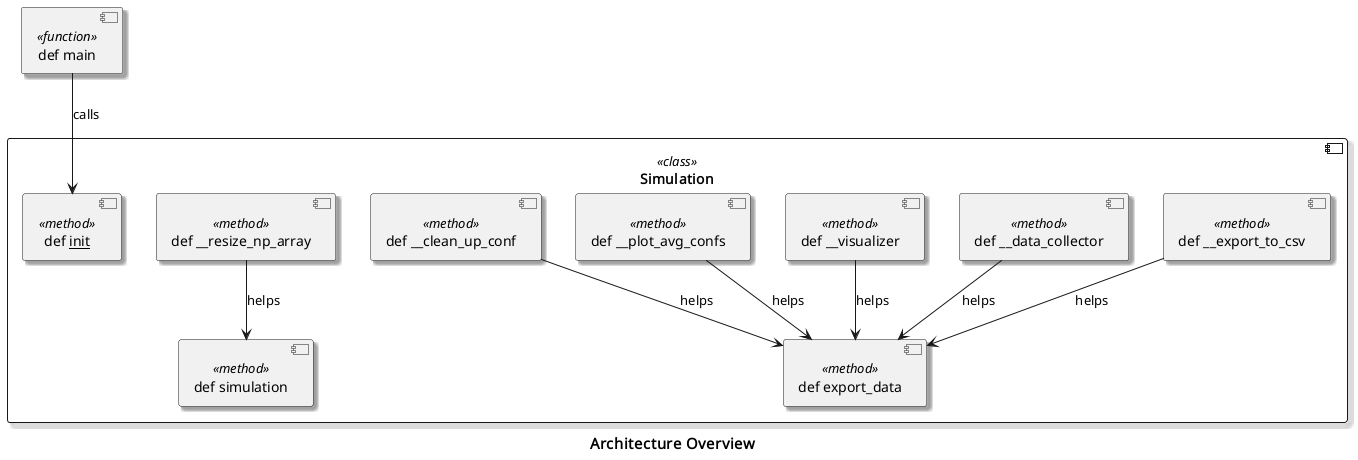
\includegraphics[scale=0.3]{B-1.png}
  \caption{Component diagram for overview of architecutre}
\end{figure}

\section{Execution Documentation}
\subsection{Summary Table}

\begin{tabular}{|l | l | l | l | l |}
  \hline
  Run ID & Purpose                                & Parameters Changed          & Duration & Status \\ [0.5ex]
  \hline\hline
  001    & Baseline                               & All defaults                & 43s      & Complete   \\
  \hline                                                                                     
  002    & Equal Contact Reduction                & s=0.70 p=0.70 a=0.70 y=0.70 & 27s      & Complete   \\
  \hline                                                                                    
  003    & Severe Equal Contact Reduction         & s=0.50 p=0.50 a=0.50 y=0.50 & 9s       & Complete   \\
  \hline                                                                                   
  004    & Symptom Contact Reduction              & y=0.70                      & 32s      & Complete   \\
  \hline                                                                                  
  005    & Severe Symptom Contact Reduction       & y=0.50                      & 32s      & Complete   \\
  \hline                                                                                 
  006    & Infectious Reduction                   & p=0.70 a=0.70 y=0.70        & 29s      & Complete   \\
  \hline                                                                                 
  007    & Severe Infectious Reduction            & p=0.50 a=0.50 y=0.50        & 24s      & Complete   \\
  \hline                                                                                 
  008    & Susceptible Reduction                  & s=0.70                      & 34s      & Complete   \\
  \hline                                                                                 
  009    & Severe Susceptible Reduction           & s=0.50                      & 32s      & Complete   \\
  \hline                                                                                 
  010    & Realistic Symptomatic Reduction        & s=0.70 p=0.70 a=0.70 y=0.50 & 27s      & Complete   \\
  \hline                                                                                 
  011    & Realistic Widespread Testing Reduction & s=0.70 p=0.50 a=0.50 y=0.50 & 12s      & Complete   \\
  \hline                                                                                 
  012    & Extreme Equal Contact Reduction        & s=0.30 p=0.30 a=0.30 y=0.30 & 2s       & Complete   \\
  \hline\hline
\end{tabular}

\subsection{Parameter Configuration}
The following parameters are used for each run unless otherwise mentioned:

\begin{tabular}{| l | l |}
  \hline
  Variable  & Default Value \\ [0.5ex]
  \hline\hline
  seed      & 123432        \\
  \hline
  N\_S0     & 5000          \\
  \hline
  N\_P0     & 1             \\
  \hline
  N\_A0     & 0             \\
  \hline
  N\_Y0     & 0             \\
  \hline
  N\_R0     & 0             \\
  \hline
  s         & 1.0           \\
  \hline
  p         & 1.0           \\
  \hline
  a         & 1.0           \\
  \hline
  y         & 1.0           \\
  \hline
  cycles    & 50            \\
  \hline
  avg\_steps & 50            \\
  \hline\hline
\end{tabular}

\subsection{Execution Environment}
The runs were executed with:
\begin{itemize}
\item Fedora Linux 42 (Workstation Edition)
\item Vterm Terminal
\item Python Virtual Environment
\item All modules listed in requirements
\end{itemize}

\section{Data Collection Overview}
\subsection{Metric Description}
\begin{tabular}{| l | l | l | l |}
  \hline
  File Type & Naming & Format & Contents \\ [0.5ex]
  \hline\hline 
  Summary & plot\_summary\_run\_XXX.png & PNG & Plot of each compartment \\
  \hline
  Summary & summary\_run\_XXX.csv & CSV & Metrics for each run \\
  \hline
  Time Series & timeseries\_N\_S\_XXX.csv & CSV & Time series for susceptible compartment \\
  \hline
  Time Series & timeseries\_N\_P\_XXX.csv & CSV & Time series for pre-symptomatic compartment \\
  \hline
  Time Series & timeseries\_N\_A\_XXX.csv & CSV & Time series for asymptomatic compartment \\
  \hline
  Time Series & timeseries\_N\_Y\_XXX.csv & CSV & Time series for symptomatic compartment \\
  \hline
  Time Series & timeseries\_N\_R\_XXX.csv & CSV & Time series for recovered compartment \\
  \hline
  Time Series & timeseries\_run\_XXX.csv & CSV & Time series for time for every compartment \\
  \hline\hline 
\end{tabular}

\subsection{Data Samples and Excerpts}
The most interesting runs summary metrics have been collected below.
\subsubsection{Summary Metrics Run 001}
\begin{tabular}{| l | l |}
  \hline
  Metric & Value \\
  \hline\hline
  Peak Infections & 1363 \\
  \hline
  Peak Time & 112479 \\
  \hline
  R0 & 4.0 \\
  \hline
  Attack Rate & 0.92 \\
  \hline
\end{tabular} 
\subsubsection{Summary Metrics Run 002}
\begin{tabular}{| l | l |}
  \hline
  Metric & Value \\
  \hline\hline
  Peak Infections & 569 \\
  \hline
  Peak Time & 181285 \\
  \hline
  R0 & 1.37 \\
  \hline
  Attack Rate & 0.66 \\
  \hline
\end{tabular} 
\subsubsection{Summary Metrics Run 010}
\begin{tabular}{| l | l |}
  \hline
  Metric & Value \\
  \hline\hline
  Peak Infections & 424 \\
  \hline
  Peak Time & 212730 \\
  \hline
  R0 & 0.98 \\
  \hline
  Attack Rate & 0.57 \\
  \hline
\end{tabular} 
\subsubsection{Summary Metrics Run 011}
\begin{tabular}{| l | l |}
  \hline
  Metric & Value \\
  \hline\hline
  Peak Infections & 150  \\
  \hline
  Peak Time &  \\
  \hline
  R0 & 0.50 \\
  \hline
  Attack Rate & 0.30 \\
  \hline
\end{tabular} 

\subsection{Visualization Data}
\subsubsection{Summary Plot Run 001}
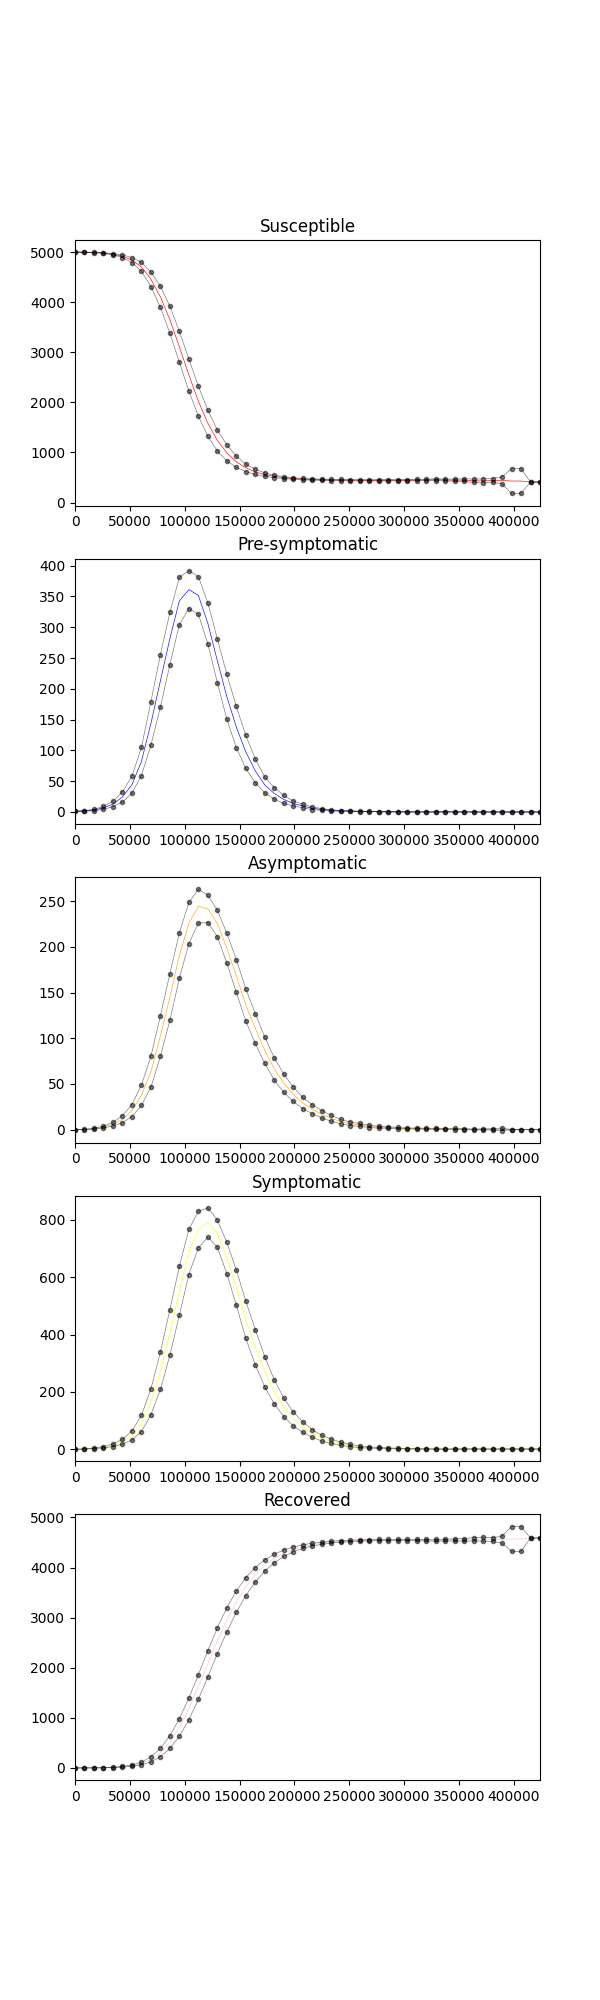
\includegraphics[scale=0.4]{plot_summary_run_001.png}
\subsubsection{Summary Plot Run 002}
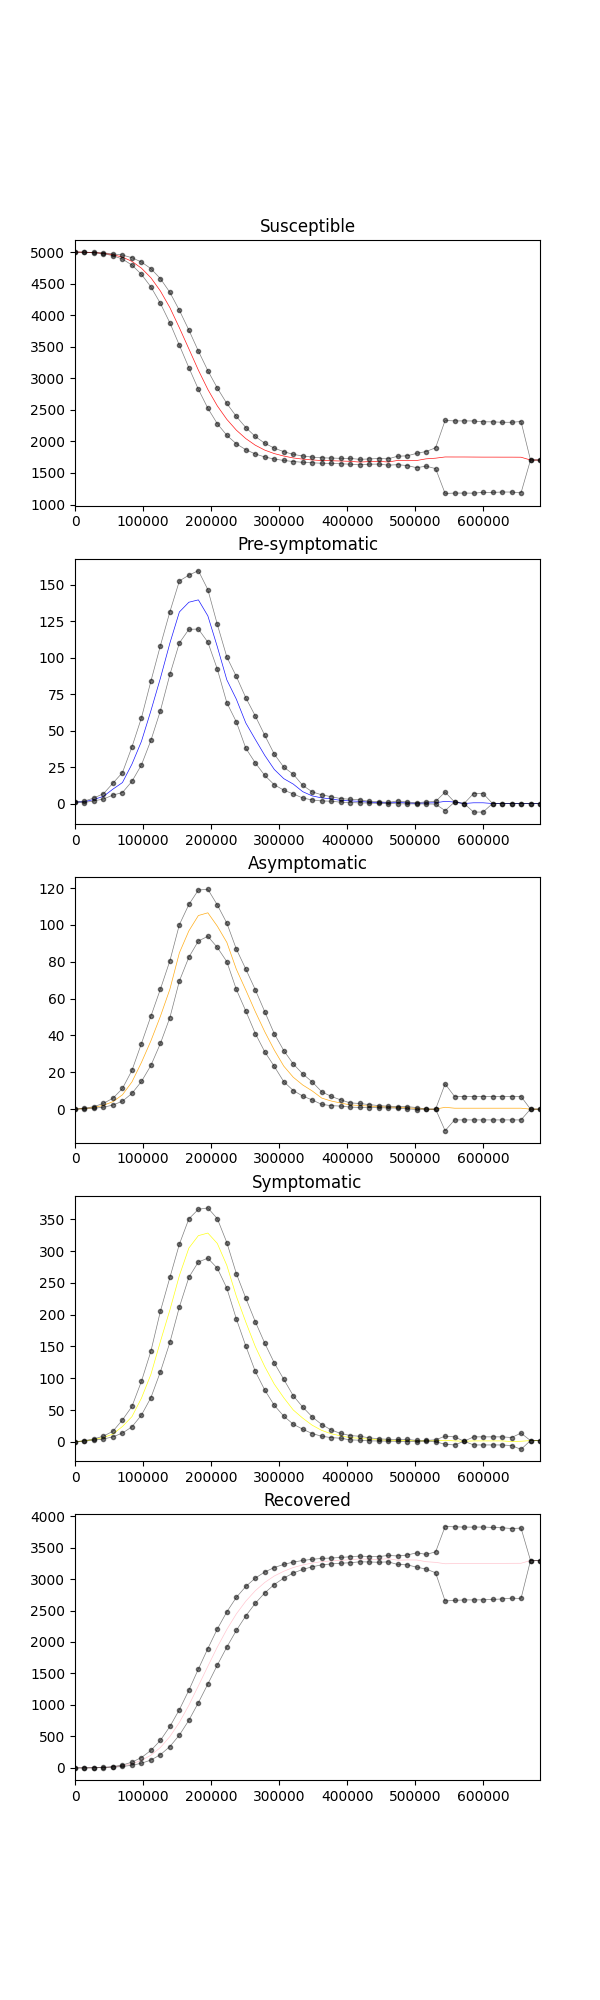
\includegraphics[scale=0.4]{plot_summary_run_002.png}
\subsubsection{Summary Plot Run 010}
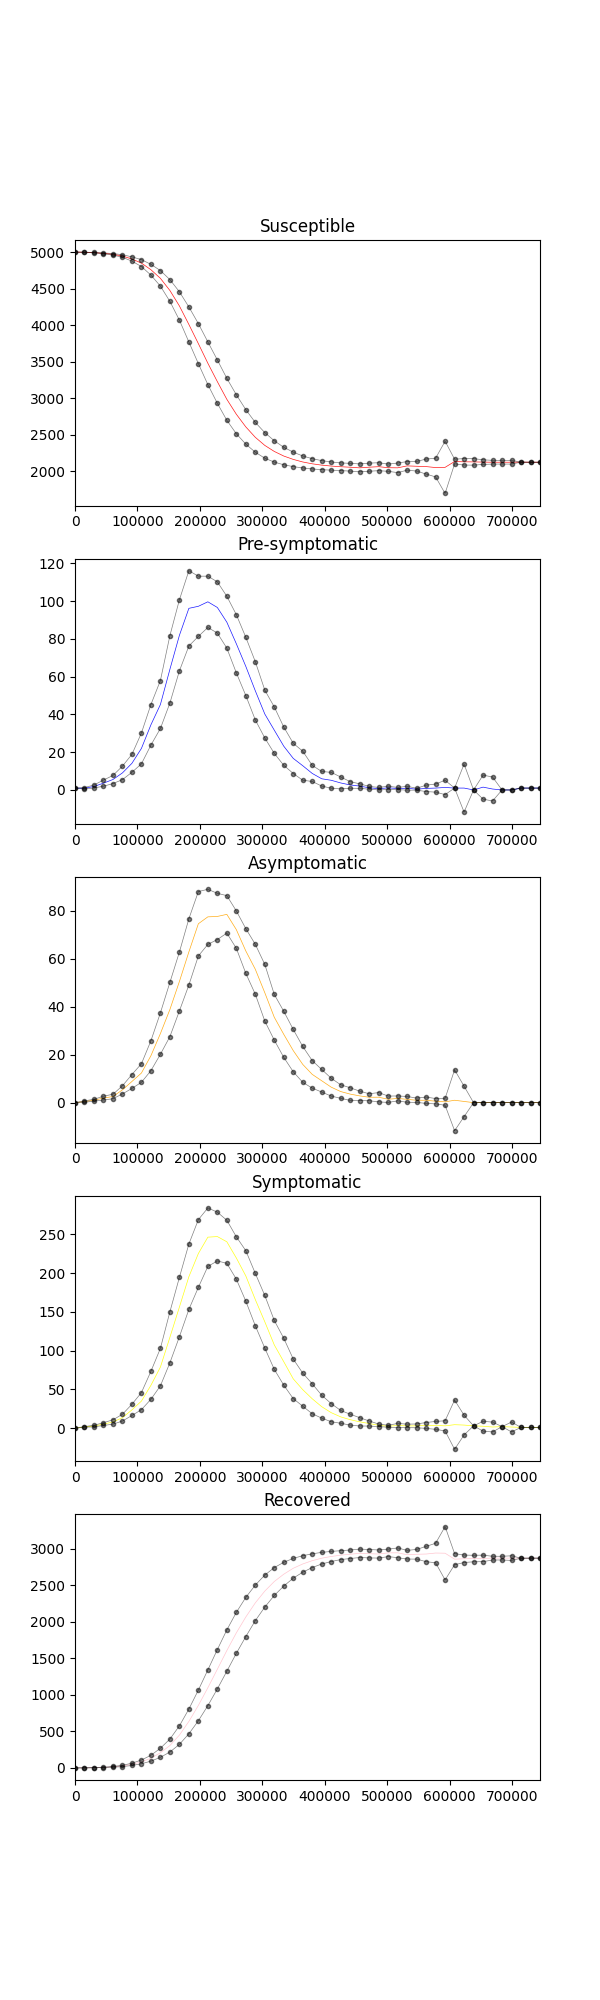
\includegraphics[scale=0.4]{plot_summary_run_010.png}
\subsubsection{Summary Plot Run 011}
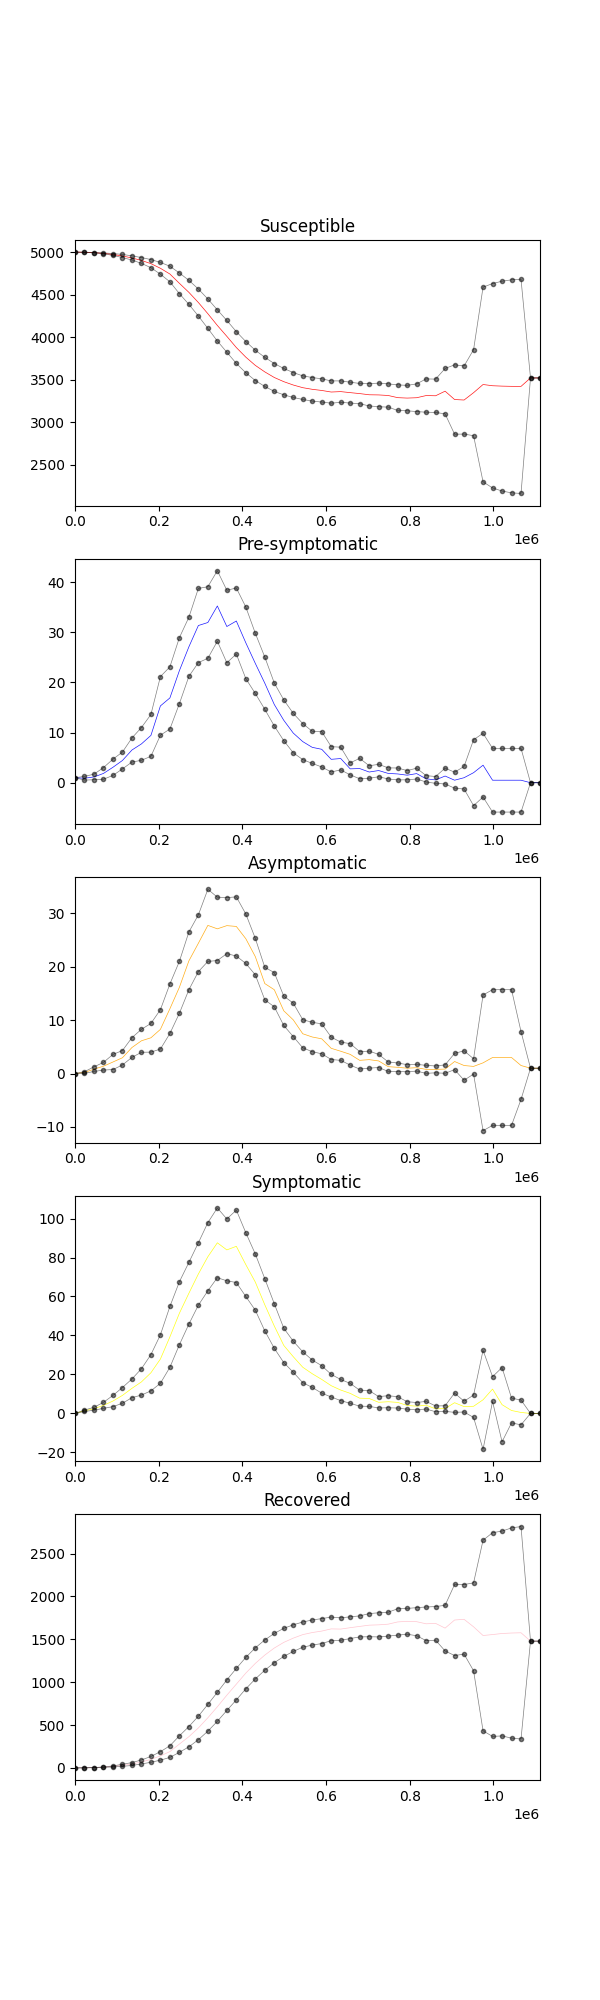
\includegraphics[scale=0.4]{plot_summary_run_011.png}

\subsection{Initial Obesrvations}
When looking at the summary metrics I observe that the peak time of infection is later the smaller the peak infection is. Also, the attack rate and R0 are clearly correlated. Furthermore, the attack rate struggles to reach a higher value than 95\%.
\newline
On the other hand, observing the plots we see that the confidence interval becomes larger the smaller the R0 is. Furthermore, It looks like the confidence interval grows larger the closer we are to the peak, and smaller the farther away we are, though at the end it enlarges which is likely due to most simulations ending before those time points.
\subsection{Preliminary Results}

\subsection{Basic Statistics}
\subsubsection{Run 001 Statistics}
\begin{tabular}{| l | l | l |}
  \hline
  Mean & Median & Mode \\
  \hline\hline
\end{tabular} 
\subsubsection{Run 002 Statistics}
\subsubsection{Run 010 Statistics}
\subsubsection{Run 011 Statistics}

\printbibliography


\end{document}
